%
% File emnlp2016.tex
%

\documentclass[11pt,letterpaper]{article}
\usepackage{emnlp2016}
\usepackage{times}
\usepackage{latexsym}
\usepackage{graphicx}
\graphicspath{ {images/} }

% Uncomment this line for the final submission:
%\emnlpfinalcopy

%  Enter the EMNLP Paper ID here:
\def\emnlppaperid{***}

% To expand the titlebox for more authors, uncomment
% below and set accordingly.
% \addtolength\titlebox{.5in}    

\newcommand\BibTeX{B{\sc ib}\TeX}


\title{Instructions for EMNLP 2016 Proceedings\Thanks{This
    document has been adapted from the instructions for earlier ACL
    and NAACL proceedings.}}

% Author information can be set in various styles:
% For several authors from the same institution:
% \author{Author 1 \and ... \and Author n \\
%         Address line \\ ... \\ Address line}
% if the names do not fit well on one line use
%         Author 1 \\ {\bf Author 2} \\ ... \\ {\bf Author n} \\
% For authors from different institutions:
% \author{Author 1 \\ Address line \\  ... \\ Address line
%         \And  ... \And
%         Author n \\ Address line \\ ... \\ Address line}
% To start a seperate ``row'' of authors use \AND, as in
% \author{Author 1 \\ Address line \\  ... \\ Address line
%         \AND
%         Author 2 \\ Address line \\ ... \\ Address line \And
%         Author 3 \\ Address line \\ ... \\ Address line}
% If the title and author information does not fit in the area allocated,
% place \setlength\titlebox{<new height>} right after
% at the top, where <new height> can be something larger than 2.25in
\author{Siddharth Patwardhan \and Daniele Pighin\\
  {\tt publication@emnlp2016.net}}

\date{}

\begin{document}

\maketitle

\begin{abstract}
  While there are gaps in our understanding of how the brain works to produce speech, existing research has shown promise that brain activity is discriminative enough for speech recognition. This study works towards multimodal speech recognition using signals from all modalities, including brain activity data through EEG, to better understand the role of each modality in speech production. We present trained models that incorporate audio, visual, and EEG information to perform phonetic-based speech recognition. We evaluate these models on phoneme classification tasks, showing separate results for speaker-dependent cases and speaker-independent cases. Classification rates indicate there are some discriminative features in visual and EEG signals but more data, further preprocessing, and more complex models may be required to effectively extract these features for speech recognition tasks.
\end{abstract}


\section{Introduction}

With the increase in computer processing speeds, there is a rising interest in convenient and accessible solutions for human-computer interaction and brain-computer interfaces. It comes as no surprise that such a solution would use speech, the most convenient form of communication for human society, as a primary means of interaction. Automatic speech recognition (ASR) has historically both relied on and driven machine learning techniques. Currently, special cases of Dynamic Bayes Networks (DBN) are popularly used for ASR models. With the advent of less invasive visual recognition technology to detect kinematic features, research has increased performance by including bimodal audio-visual observations in models to train ASR systems [1]. Although these models are implemented in many popular software solutions for the average consumer, further challenges arise when models have to account for speech disorders related to the physical production of speech. Classification boundaries for phonological categories or vocal tract movements become less obvious and recognition performance drops.

This research modeled facial tracking, audio, and EEG observations using machine learning models to relate the three modalities to each other during actual speech production, going beyond the bimodal audio-visual ASR systems. Necessary data for all three modalities previously existed and was originally used for binary classification of phonological categories. The KARAONE data set contains all three modalities at various states (silent speech state, stimulus state, speech production state) which made it highly suitable for comparing multimodal relationships without bias. Initially, relevant features from audio-visual as well as the continuous EEG recordings were extracted. Afterwards, various model architectures were experimented with to formulate and validate a model that best fits the KARA ONE dataset [2]. The models were then investigated on their performance in terms of their classification rates. The models helped in exploring multimodal relationships that can make meaningful contributions to various aspects of ASR.  The study was a step towards a better understanding of relationships between the relevant modalities and to provide additional support for ASR systems related to silent speech recognition, and brain-computer interfaces.

\section{Literature Review}

\subsection{Dynamic Bayesian Networks}
In the early 1990s, Paul Dagum developed the concept of Dynamic Bayes Networks [3] (DBNs) – calling them Dynamic Network Models – which can be seen as generalizing some of the more simple models for sequential data analysis like Hidden Markov Models (HMMs) [4]. DBNs are a form of traditional Bayesian probabilistic graphical models that represent conditional dependencies between random variables by using directed acyclic graphs. Various algorithms can use these models for supervised learning and inference by supplying them with evidence and historical data. DBNs, today, are applied to a variety of applications including the primary interest of this paper, multi-modal speech recognition [4]. Generally, for speech recognition, the sequential data comes in the form of temporal (time-series) data and subsequent models will therefore attempt to capture the forward moving linearity of time. Firstly, using just a static network, we can capture contemporaneous dependencies between variables, and then expand it into a dynamic network which will model these dependencies across time (Figure 2.1) [3]. The static network can be considered as a single time-slice in a DBN, which then links a time-slice to the next using directed (since we are dealing with temporal sequence data) arcs between them [5]. In this sense, DBN becomes an acyclic graph with edges representing dependencies between the vertices or variables [4]. It is important to note that the static network graph structure for each time slice does not change over time [5], as Dagum’s motivation for DBNs was simply to forecast future values of variables given the structure of the static network [3].

\begin{figure}[ht]
\centering
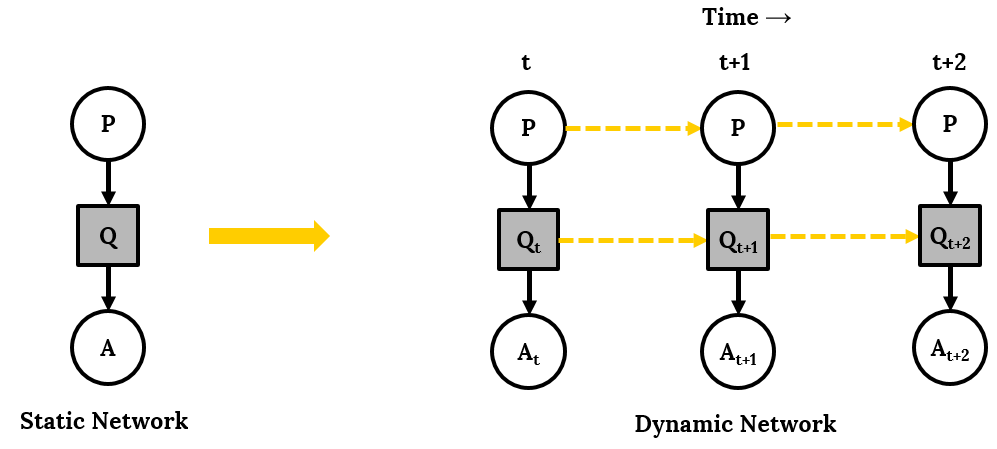
\includegraphics[scale=0.25]{dbn_description}
\caption{DBN Overview}
\end{figure}

To better understand the advantages and disadvantages of DBNs, we can start by observing HMMs, a specific case of DBNs. A simple variant – there are more complicated versions which still fall under the DBN generalization – of an HMM represents the hidden state of the world using a single discrete random variable, $X_t$, which can take on various values [5]. The hidden state can be considered to generate an observation (represented by an arc leading from the former to the latter) which is modeled by another random variable, $Y_t$ . The directed relationship between $X_t$ and $Y_t$ can be considered a single time slice or the static network. Placing a directed arc between the hidden states of one time slice to the next (e.g. $X_1$ to $X_2$) will form a dynamic network [3]. Figure 2.2 depicts a simple HMM as described above. Similarly, we can form a graph with more than one variable to represent the hidden state and more than one variable to represent the observed state, generalizing the HMM to a DBN [5].To better understand the advantages and disadvantages of DBNs, we can start by observing HMMs, a specific case of DBNs. A simple variant – there are more complicated versions which still fall under the DBN generalization – of an HMM represents the hidden state of the world using a single discrete random variable, $X_t$, which can take on various values [5]. The hidden state can be considered to generate an observation (represented by an arc leading from the former to the latter) which is modeled by another random variable, $Y_t$ . The directed relationship between $X_t$ and $Y_t$ can be considered a single time slice or the static network. Placing a directed arc between the hidden states of one time slice to the next (e.g. $X_1$ to $X_2$) will form a dynamic network [3]. Figure 2.2 depicts a simple HMM as described above. Similarly, we can form a graph with more than one variable to represent the hidden state and more than one variable to represent the observed state, generalizing the HMM to a DBN [5].

\section{Data}

The database – KARAONE [2] – used for this study is available to the public and contains all three modalities that are of interest to this paper – audio-visual data as well as complimentary EEG data. All three modalities were collected during a stimulus state – prompt text appeared on screen –, a silent/imagine speech state – participant imagined speaking the prompt without actual production –, and a speaking stage – where the participant spoke the prompt out loud [2]. Data is available for 14 participants who were prompted 12 times for each of the 11 prompts (a total of 132 trial for each participant), which were a mix of phonemic and isolated word prompts. The study, concerned with end-to-end learning of phonetic-based ASR, dealt with only the 7 phonemic prompts (/uw/, /tiy/, /iy/, /m/, /n/, /piy/, /diy/). 

The KARAONE [2] database has certain advantages that makes it suitable for our purposes. Since we are primarily concerned with finding multi-modal relationships that can benefit speech recognition or brain-computer interfaces, the methods through which data was collected are advantageous. Visual data is collected using relatively simple means through a consumer product [2] which makes it feasible to use for modeling practical conditions. Furthermore, accessing language centers directly can be invasive to achieve ideal and high SNRs [15, 2] but EEG recordings are a more accessible and applicable solution [15, 2], and by definition, non-invasive. Once again, for our purposes, working with data that is more accessible is advantageous since general brain-computer interfaces or ASR systems will not have access to more intrusive methods, even if they can provide less noisy data. Furthermore, the KARAONE database contains data from both silent speech and spoken speech states [2] for the same prompts which is ideal for our purpose of determining multi-modal relationships. Access to neural activity relatively uncontaminated by physiological artifacts [14, 15] allows us to make unbiased comparisons with audio-visual modalities. Lastly, since the database contains data from multiple speakers, it allows this study to explore speaker-independent multi-modal speech recognition as well.  

\subsection{Audio Data}
Audio Data was available in the form of .wav files, sampled at 16 KHz and each trail separated into a unique file. Each of these audio segments were converted into 42 dimension vectors of Mel-Frequency Cepstral Coefficients (MFCC) across time using VOICEBOX [19], a speech processing toolbox for MATLAB under a GNU Public license.

\subsection{Visual Data}
The visual data in the database used a Microsoft Kinect camera [20] to record the participants during trials. For each frame of the captured video, 6 Animation Units (AUs) – ranging between -1 to +1 – were extracted corresponding to Figure 3.1. AU values were obtained from .AU files within the database and could be up-sampled such that both the Visual data and the MFCC data had the same total number of time slices for each trial. At each time-slice, the visual data consisted of a 6-dimension vector.

\subsection{EEG Data}
EEG data was available in the form of a .cnt file in the database [2], from which continuous 64-dimension (one for each electrode) data was extracted using EEGLAB, an open source MATLAB environment for electrophysiological signal processing [21].  Only 10 of the 64 channels were used as training data as they proved to be the most discriminative features from previous research [2]. The electrode positioning followed the 10-20 system, see Figure 2.7. Note that we are working with EEG data during the imagined/silence speech state since during other stages, the recording contain a large amount of artifacts (e.g. from screen, muscle movement, etc.).

\section{Methodology}
This study designed and trained models incorporating information from all relevant modalities. Using 9-fold cross validation for speaker dependent speech recognition models and 10-fold cross validation for speaker independent speech recognition models, the models were evaluated by their classification rates. The design, creation, and training of the models is discussed in the following sub sections. 

\subsection{DBN Design}
Dynamic Bayes Networks were designed in MATLAB for this study, using Kevin Murphy’s open source Bayes Net Toolbox (BNT) [22]. BNT supports not only the design of DBNs but also supports many inference algorithms and methods (Figure 2.3). Two separate DBNs were designed, one for EEG modeling, the other incorporating audio-visual modes. Since the EEG data being used is during the ‘silent-speech’ state, it is not synchronous with the audio-visual data which is for the ‘speech-production’ state and a separate DBN for the EEG mode was necessary.

Our EEG DBN, depicted in Figure 4.1, is defined as a GMM-HMM, where a Gaussian mixture model, with 12 multivariate Gaussians, occupies a node. Otherwise, the phoneme (P) and hidden state (Q) nodes are discrete nodes while node E contains the continuous observed EEG feature vectors at each time step. The only interdependencies across time steps is a connection between the hidden nodes.

The audio-visual DBN (Figure 4.2) models phonemes (P), visual data (V), and the hidden state (Q) with discrete nodes while node A contains continuous observed MFCC coefficients across time steps. The visual data, up-sampled to match the temporal length of our audio data, is preprocessed with K-means algorithm into clusters to convert it from continuous to discrete. As visible in Figure 4.2, the audio data is conditionally dependent on all other nodes while the visual data is only conditionally dependent on nodes P and Q. Theoretically, this models the dependency of the produced speech on the positions of certain facial features (e.g. curve of the lips). 

Final classifications were performed by taking into account the likelihood of test data being generated by a certain phoneme, for each DBN. 

\begin{figure}[h]
\centering
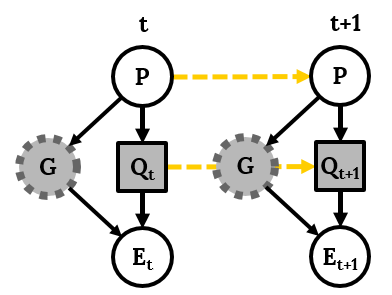
\includegraphics[scale=0.5]{dbn_design_eeg}
\caption{EEG DBN Design}
\end{figure}

\begin{figure}[h]
\centering
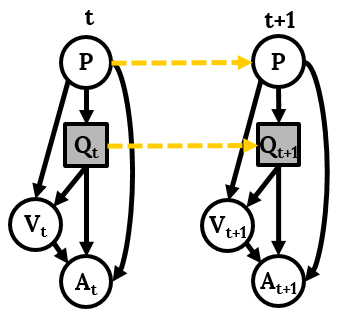
\includegraphics[scale=0.5]{dbn_design_audio}
\caption{Audio-visual DBN Design}
\end{figure}

\subsection{RNN Design}
The second approach to multi-modal speech recognition in this study involved the use of recurrent neural networks to capture temporal dependencies for each mode and integrate the modes together to train a multi-layer perceptron. Figure 4.3 illustrates the complete architecture for training our multi-modal phoneme classifier. The training data ($x_A,x_V,x_E$) – 42-dimension audio MFCCs, 6-dimension visual Kinect AU units, 10-dimension raw EEG data – for each RNN consisted of the data for each mode labeled with the respective phoneme. The hidden units of the RNNs were LSTM cells to increase memory of model. Figure 4.4 shows the final parameters used for training after various trials and error to determine those resulting in best performance. Once each separate RNN model was trained, the output of the hidden layer in the last time step $(h_A^((T_A ) ),h_V^((T_V ) ),h_E^((T_E ) ))$ for each training case was taken as training data for a multi-layer perceptron, consisting of sigmoid activations. These architectures were designed and coded using Theano in python.

\begin{figure}[h]
\centering
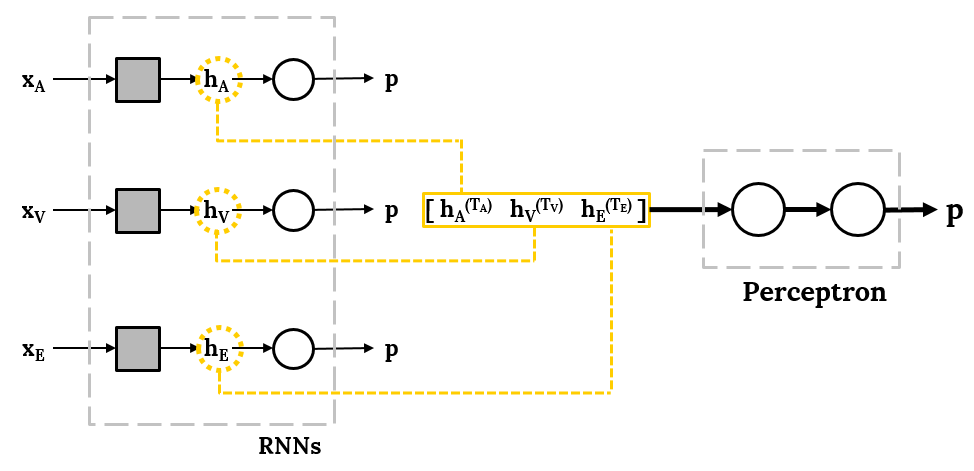
\includegraphics[scale=0.25]{rnn_design}
\caption{RNN Architecture}
\end{figure}


\section{General Instructions}



Manuscripts must be in two-column format.  Exceptions to the two-column
format include the title, as well as the authors' names and complete
addresses (only in the final version, not in the version submitted for
review), which must be centered at the top of the first page (see the
guidelines in Subsection~\ref{ssec:first}), and any full-width figures or
tables.  Type single-spaced.  Do not number the pages in the camera-ready
version. Start all pages directly under the top margin.  See the guidelines
later regarding formatting the first page.  Also see 
Section~\ref{sec:length} for the page limits.

By uncommenting {\small\verb|\emnlpfinalcopy|} at the top of this document,
it will compile to produce an example of the camera-ready formatting; by
leaving it commented out, the document will be anonymized for initial
submission.  When you first create your submission on softconf, please fill
in your submitted paper ID where {\small\verb|***|} appears in the
{\small\verb|\def\emnlppaperid{***}|} definition at the top.

The review process is double-blind, so do not include any author information
(names, addresses) when submitting a paper for review. However, you should
maintain space for names and addresses so that they will fit in the final
(accepted) version.  The EMNLP 2016 \LaTeX\ style will create a titlebox
space of 2.5in for you when {\small\verb|\emnlpfinalcopy|} is commented out.

\subsection{The Ruler}
The EMNLP 2016 style defines a printed ruler which should be present in the
version submitted for review.  The ruler is provided in order that
reviewers may comment on particular lines in the paper without
circumlocution.  If you are preparing a document without the provided
style files, please arrange for an equivalent ruler to
appear on the final output pages.  The presence or absence of the ruler
should not change the appearance of any other content on the page.  The
camera ready copy should not contain a ruler. (\LaTeX\ users may uncomment
the {\small\verb|\emnlpfinalcopy|} command in the document preamble.)  

Reviewers:
note that the ruler measurements do not align well with lines in the paper
--- this turns out to be very difficult to do well when the paper contains
many figures and equations, and, when done, looks ugly.  Just use fractional
references (e.g., the first line on this page is at mark $096.5$), although
in most cases one would expect that the approximate location will be
adequate.

\subsection{Electronically-Available Resources}

EMNLP provides this description to authors in \LaTeX2e{} format
and PDF format, along with the \LaTeX2e{} style file used to format it
({\small\tt emnlp2016.sty}) and an ACL bibliography style
({\small\tt emnlp2016.bst}) and example bibliography
({\small\tt emnlp2016.bib}). A Microsoft Word template file
({\small\tt emnlp2016.dotx}) is also available. We strongly recommend the
use of these style files, which have been appropriately tailored for the
EMNLP 2016 proceedings.

\subsection{Format of Electronic Manuscript}
\label{sect:pdf}

For the production of the electronic manuscript, you must use Adobe's
Portable Document Format (PDF). This format can be generated from
postscript files: on Unix systems, you can use {\small\tt ps2pdf} for this
purpose; under Microsoft Windows, you can use Adobe's Distiller, or
if you have cygwin installed, you can use {\small\tt dvipdf} or
{\small\tt ps2pdf}.  Note 
that some word processing programs generate PDF that may not include
all the necessary fonts (esp.\ tree diagrams, symbols). When you print
or create the PDF file, there is usually an option in your printer
setup to include none, all, or just non-standard fonts.  Please make
sure that you select the option of including ALL the fonts.  {\em Before
sending it, test your {\/\em PDF} by printing it from a computer different
from the one where it was created}. Moreover, some word processors may
generate very large postscript/PDF files, where each page is rendered as
an image. Such images may reproduce poorly.  In this case, try alternative
ways to obtain the postscript and/or PDF.  One way on some systems is to
install a driver for a postscript printer, send your document to the
printer specifying ``Output to a file'', then convert the file to PDF.

For reasons of uniformity, Adobe's {\bf Times Roman} font should be
used. In \LaTeX2e{} this is accomplished by putting
\small
\begin{verbatim}
\usepackage{times}
\usepackage{latexsym}
\end{verbatim}
\normalsize
in the preamble.
Additionally, it is of utmost importance to specify the {\bf US-Letter
format} (8.5in $\times$ 11in) when formatting the paper. When working with
{\small\tt dvips}, for instance, one should specify {\small\tt -t letter}.

Print-outs of the PDF file on US-Letter paper should be identical to the
hardcopy version.  If you cannot meet the above requirements about the
production of your electronic submission, please contact the
publication chairs above  as soon as possible.

\subsection{Layout}
\label{ssec:layout}

Format manuscripts with two columns to a page, following the manner in
which these instructions are formatted. The exact dimensions for a page
on US-Letter paper are:

\begin{itemize}
\item Left and right margins: 1 inch
\item Top margin: 1 inch
\item Bottom margin: 1 inch
\item Column width: 3.15 inches
\item Column height: 9 inches
\item Gap between columns: 0.2 inches
\end{itemize}

\noindent Papers should not be submitted on any other paper size.
Exceptionally, authors for whom it is \emph{impossible} to format on
US-Letter paper may format for \emph{A4} paper. In this case, they should
keep the \emph{top} and \emph{left} margins as given above, use the same
column width, height and gap, and modify the bottom and right margins as
necessary. Note that the text will no longer be centered.

\subsection{The First Page}
\label{ssec:first}

Center the title, author name(s) and affiliation(s) across both
columns (or, in the case of initial submission, space for the names). 
Do not use footnotes for affiliations.  
Use the two-column format only when you begin the abstract.

\noindent{\bf Title}: Place the title centered at the top of the first
page, in a 15 point bold font.  (For a complete guide to font sizes and
styles, see Table~\ref{font-table}.) Long titles should be typed on two
lines without a blank line intervening. Approximately, put the title at
1in from the top of the page, followed by a blank line, then the author
name(s), and the affiliation(s) on the following line.  Do not use only
initials for given names (middle initials are allowed). Do not format
surnames in all capitals (e.g., ``Mitchell,'' not ``MITCHELL'').  The
affiliation should contain the author's complete address, and if possible,
an email address. Leave about 0.75in between the affiliation and the body
of the first page.

\noindent{\bf Abstract}: Type the abstract at the beginning of the first
column.  The width of the abstract text should be smaller than the
width of the columns for the text in the body of the paper by about
0.25in on each side.  Center the word {\bf Abstract} in a 12 point
bold font above the body of the abstract. The abstract should be a
concise summary of the general thesis and conclusions of the paper.
It should be no longer than 200 words.  The abstract text should be in
10 point font.

\begin{table}
\centering
\small
\begin{tabular}{cc}
\begin{tabular}{|l|l|}
\hline
{\bf Command} & {\bf Output}\\\hline
\verb|{\"a}| & {\"a} \\
\verb|{\^e}| & {\^e} \\
\verb|{\`i}| & {\`i} \\ 
\verb|{\.I}| & {\.I} \\ 
\verb|{\o}| & {\o} \\
\verb|{\'u}| & {\'u}  \\ 
\verb|{\aa}| & {\aa}  \\\hline
\end{tabular} & 
\begin{tabular}{|l|l|}
\hline
{\bf Command} & {\bf  Output}\\\hline
\verb|{\c c}| & {\c c} \\ 
\verb|{\u g}| & {\u g} \\ 
\verb|{\l}| & {\l} \\ 
\verb|{\~n}| & {\~n} \\ 
\verb|{\H o}| & {\H o} \\ 
\verb|{\v r}| & {\v r} \\ 
\verb|{\ss}| & {\ss} \\\hline
\end{tabular}
\end{tabular}
\caption{Example commands for accented characters, to be used in, e.g., \BibTeX\ names.}\label{tab:accents}
\end{table}

\noindent{\bf Text}: Begin typing the main body of the text immediately
after the abstract, observing the two-column format as shown in the present
document. Do not include page numbers in the camera-ready manuscript.  

Indent when starting a new paragraph. For reasons of uniformity,
use Adobe's {\bf Times Roman} fonts, with 11 points for text and 
subsection headings, 12 points for section headings and 15 points for
the title.  If Times Roman is unavailable, use {\bf Computer Modern
  Roman} (\LaTeX2e{}'s default; see section \ref{sect:pdf} above).
Note that the latter is about 10\% less dense than Adobe's Times Roman
font.

\subsection{Sections}

\noindent{\bf Headings}: Type and label section and subsection headings in
the style shown on the present document.  Use numbered sections (Arabic
numerals) in order to facilitate cross references. Number subsections
with the section number and the subsection number separated by a dot,
in Arabic numerals. 

\noindent{\bf Citations}: Citations within the text appear in parentheses
as~\cite{Gusfield:97} or, if the author's name appears in the text itself,
as Gusfield~\shortcite{Gusfield:97}.  Using the provided \LaTeX\ style, the
former is accomplished using {\small\verb|\cite|} and the latter with
{\small\verb|\shortcite|} or {\small\verb|\newcite|}.  Collapse multiple
citations as in~\cite{Gusfield:97,Aho:72}; this is accomplished with the
provided style using commas within the {\small\verb|\cite|} command, e.g.,
{\small\verb|\cite{Gusfield:97,Aho:72}|}. Append lowercase letters to the
year in cases of ambiguities. Treat double authors as in~\cite{Aho:72}, but
write as in~\cite{Chandra:81} when more than two authors are involved.  

\noindent{\bf References}:  We recommend
including references in a separate~{\small\texttt .bib} file, and include
an example file in this release ({\small\tt naalhlt2016.bib}). Some commands
for names with accents are provided for convenience in
Table~\ref{tab:accents}. References stored in the separate~{\small\tt .bib}
file are inserted into the document using the following commands:

\small
\begin{verbatim}
\bibliography{emnlp2016}
\bibliographystyle{emnlp2016}
\end{verbatim}
\normalsize 

References should appear under the heading {\bf References} at the end of
the document, but before any Appendices, unless the appendices contain
references. Arrange the references alphabetically by first author, rather
than by order of occurrence in the text.
% This behavior is provided by default in the provided \BibTeX\ style
% ({\small\tt emnlp2016.bst}). 
Provide as complete a reference list as possible, using a consistent format,
such as the one for {\em Computational Linguistics\/} or the one in the 
{\em Publication Manual of the American Psychological Association\/}
\cite{APA:83}. Authors' full names rather than initials are preferred. You
may use {\bf standard} abbreviations for conferences\footnote{\scriptsize {\tt https://en.wikipedia.org/wiki/ \\ \-\hspace{.75cm} List\_of\_computer\_science\_conference\_acronyms}}
and journals\footnote{\tt http://www.abbreviations.com/jas.php}.

\noindent{\bf Appendices}: Appendices, if any, directly follow the text and
the references (unless appendices contain references; see above). Letter
them in sequence and provide an informative title: {\bf A. Title of Appendix}.

\noindent{\bf Acknowledgments}: A section for acknowledgments to funding
agencies, colleagues, collaborators, etc. should go as a last (unnumbered)
section immediately before the references. Keep in mind that, during review,
anonymization guidelines apply to the contents of this section too.
% In general, to maintain anonymity, refrain from including acknowledgments in
% the version of the paper submitted for review.  

\subsection{Footnotes}

\noindent{\bf Footnotes}: Put footnotes at the bottom of the page. They may be
numbered or referred to by asterisks or other symbols.\footnote{This is
how a footnote should appear.} Footnotes should be separated from the text
by a line.\footnote{Note the line separating the footnotes from the text.}
Footnotes should be in 9 point font.

\subsection{Graphics}

\noindent{\bf Illustrations}: Place figures, tables, and photographs in the
paper near where they are first discussed, rather than at the end, if possible.
Wide illustrations may run across both columns and should be placed at the
top of a page. Color illustrations are discouraged, unless you have verified
that they will be understandable when printed in black ink. 

\begin{table}
\small
\centering
\begin{tabular}{|l|rl|}
\hline \bf Type of Text & \bf Font Size & \bf Style \\ \hline
paper title & 15 pt & bold \\
author names & 12 pt & bold \\
author affiliation & 12 pt & \\
the word ``Abstract'' & 12 pt & bold \\
section titles & 12 pt & bold \\
document text & 11 pt  &\\
abstract text & 10 pt & \\
captions & 9 pt & \\
caption label & 9 pt & bold \\
bibliography & 10 pt & \\
footnotes & 9 pt & \\
\hline
\end{tabular}
\caption{\label{font-table} Font guide.}
\end{table}

\noindent{\bf Captions}: Provide a caption for every illustration; number each one
sequentially in the form:  ``{\bf Figure 1:} Figure caption.'',
``{\bf Table 1:} Table caption.''  Type the captions of the figures and tables
below the body, using 9 point text. Table and Figure labels should be
bold-faced.

\subsection{Accessibility}
\label{ssec:accessibility}

In an effort to accommodate the color-blind (and those printing to paper),
grayscale readability of papers is encouraged. Color is not forbidden, but 
authors should ensure that tables and figures do not rely solely on color to
convey critical distinctions.

\section{Length of Submission}
\label{sec:length}

The EMNLP 2016 main conference accepts submissions of long papers and
short papers.  Long papers may consist of up to eight (8) pages of content, plus
two (2) pages for references. Upon acceptance, final versions of long papers
will be given one additional page (i.e., up to 9 pages) for content, with
unlimited pages for references --- so that reviewers' comments can be taken
into account.  Short papers may consist of up to four (4) pages of content,
plus two (2) pages for references. Upon acceptance, the final version of
short papers will be given five (5) pages in the proceedings, with unlimited
pages for references.  For both long and short papers, all illustrations and
appendices must be accommodated within these page limits, observing the
formatting instructions given in the present document.  Papers that do not
conform to the specified length and formatting requirements are subject to
be rejected without review.

EMNLP 2016 encourages submitting software and data that is described in the
paper as supplementary material. EMNLP 2016 also encourages reporting
preprocessing decisions, model parameters, and other details necessary for the
exact replication of the experiments described in the paper. Papers may be
accompanied by supplementary material, consisting of software, data, pseudo-code,
detailed proofs or derivations that do not fit into the paper, lists of features
or feature templates, parameter specifications, and sample inputs and outputs
for a system. The paper should not rely on the supplementary material: while the
paper may refer to and cite the supplementary material and the supplementary
material will be available to reviewers, they will not be asked to review the
supplementary material.

\section{Double-Blind Review Process}
\label{sec:blind}

As the reviewing will be blind, the paper must not include the authors' names and
affiliations.  Furthermore, self-references that reveal the authors' identity,
e.g., ``We previously showed (Smith,1991) ...'' must be avoided. Instead, use
citations such as ``Smith previously showed (Smith, 1991) ...'' Papers that do
not conform to these requirements will be rejected without review. In addition,
please do not post your submissions on the web until after the review process is
complete (in special cases this is permitted: see the multiple submission policy
below).

We will reject without review any papers that do not follow the official style
guidelines, anonymity conditions and page limits.

\section{Multiple Submission Policy}

Papers that have been or will be submitted to other meetings or publications must
indicate this at submission time, and must be withdrawn from the other venues if
accepted by EMNLP 2016. We will not accept for publication or presentation papers
that overlap significantly in content or results with papers that will be (or
have been) published elsewhere. Authors submitting more than one paper to EMNLP
2016 must ensure that submissions do not overlap significantly (\textgreater~25\%) with
each other in content or results.

Preprint servers such as arXiv.org and workshops that do not have
published proceedings are not considered
archival for purposes of submission. Authors must state in the online submission
form the name of the workshop or preprint server and title of the non-archival
version. The submitted version should be suitably anonymized and not contain
references to the prior non-archival version. Reviewers will be told: ``The
author(s) have notified us that there exists a non-archival previous version of
this paper with significantly overlapping text. We have approved submission under
these circumstances, but to preserve the spirit of blind review, the current
submission does not reference the non-archival version.'' Reviewers are free to do
what they like with this information.

All accepted papers must be presented at the conference to appear in the
proceedings. At least one author of each accepted paper must register for EMNLP
2016. Accepted papers will be presented orally or as a poster, at the discretion
of the program chairs (based on the nature rather than the quality of the work).
There will be no distinction in the proceedings between papers presented orally
or as posters.

\section*{Acknowledgments}

Do not number the acknowledgment section.

\bibliography{emnlp2016}
\bibliographystyle{emnlp2016}

\end{document}
